\chapter{Generative Adversarial Networks}

Le \textbf{Generative Adversarial Networks} (GAN), introdotte da \textit{Ian Goodfellow} nel 2014~\cite{goodfellow2014generative}, rappresentano una delle nuove idee nel campo dell’Intelligenza Artificiale. Si tratta di una classe di reti neurali progettate per generare dati nuovi e realistici, a partire da esempi osservati. Alla base della generazione di dati realistici c’è sempre un processo di trasformazione di semplici variabili casuali (spesso uniformi) in variabili complesse. Nonostante i calcolatori siano sistemi \textbf{deterministici} (dato un input, producono sempre lo stesso output), è comunque possibile costruire algoritmi capaci di generare sequenze numeriche che si comportano similmente a sequenze casuali. Questi algoritmi, detti \textbf{Pseudo-Random Generators}, permettono di produrre numeri che approssimano una distribuzione uniforme sull’intervallo $[0,1]$. A partire da questa base, esistono diverse tecniche per ottenere variabili casuali con distribuzioni sempre più sofisticate. Tutti questi metodi sfruttano "trucchi" matematici diversi, ma condividono un'idea comune: ottenere variabili casuali complesse come risultato di una trasformazione applicata a variabili semplici.

\section{La Trasformazione Inversa}

Una tecnica semplice è il metodo della trasformazione inversa. Supponiamo di voler generare una variabile casuale $X$ che segua una distribuzione con funzione di distribuzione cumulativa $F_X(x)$. L’idea è partire da una variabile casuale $u$ distribuita uniformemente in $\mathcal{U}(0,1)$, e ottenere $x$ tramite:
\begin{equation}
    x = F_X^{-1}(u)
\end{equation}
In questo modo, $x$ sarà distribuito secondo la legge desiderata. L’idea si può estendere anche a funzioni di trasformazione generali, che mappano variabili semplici (non necessariamente uniformi) in variabili con una distribuzione target.

\begin{figure}
    \centering
    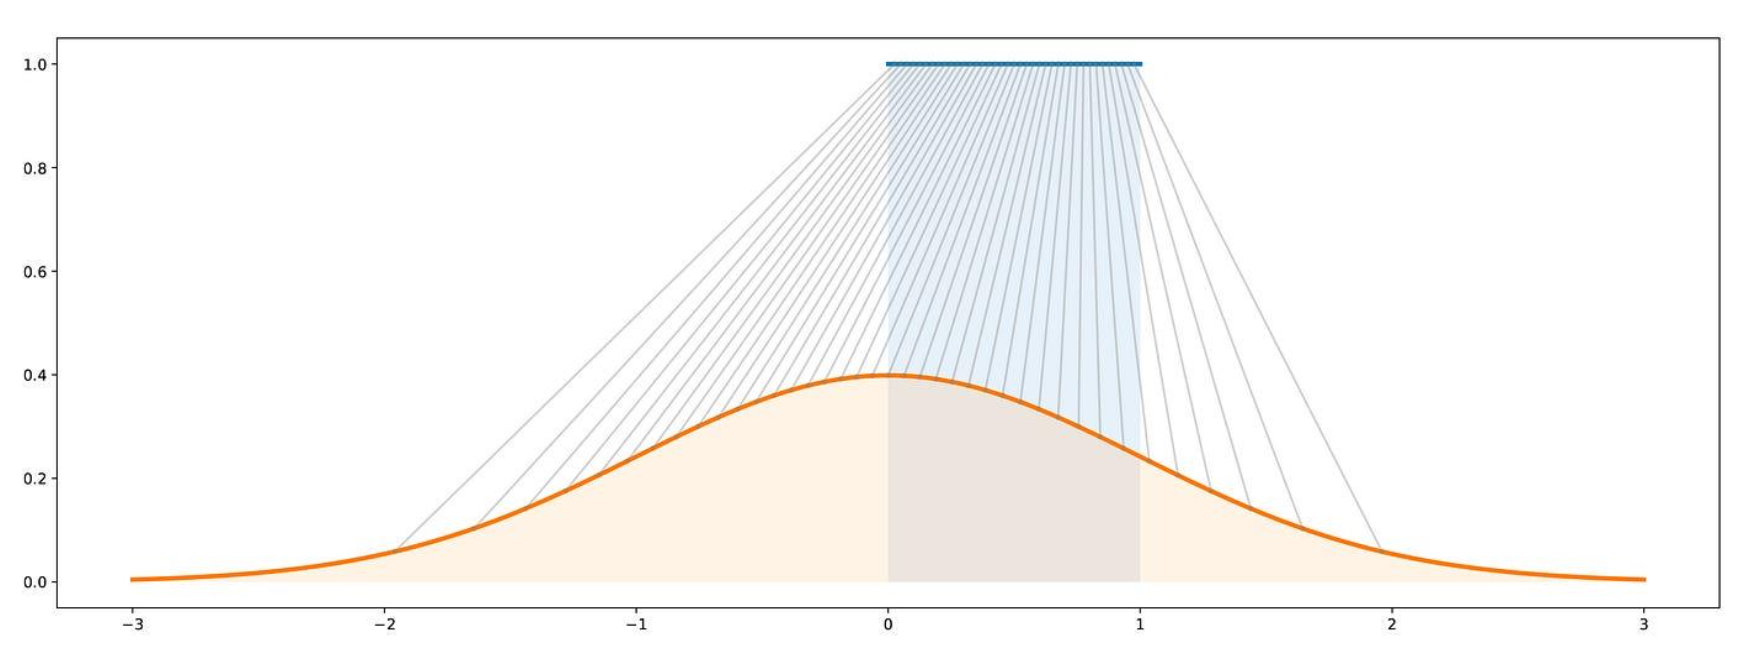
\includegraphics[width=\textwidth]{figure/InvTrasf.png}
    \caption{In blu, la distribuzione uniforme su $[0,1]$; in arancione, una distribuzione gaussiana standard; in grigio, le linee che mostrano la mappatura dalla distribuzione uniforme a quella gaussiana.}
    \label{fig:invTrasf}
\end{figure}

\section{Modelli Generativi}

Se volessimo generare immagini in bianco e nero di cani, con dimensione $n \times n$ pixel. Ogni immagine può essere "linearizzata" in un vettore $N$ di lunghezza $n^2$, mettendo le colonne una sopra l’altra. In questo modo, ogni immagine può essere rappresentata da un punto nello spazio vettoriale $\mathbb{R}^N$. Ma attenzione: non tutti i vettori in $\mathbb{R}^N$ rappresentano cani. Solo una piccola regione di questo spazio contiene vettori che corrispondono a immagini di cani, possiamo allora immaginare l’esistenza di una distribuzione di probabilità su $\mathbb{R}^N$, che chiameremo "distribuzione dei cani", la quale assegna alta probabilità ai vettori che rappresentano immagini realistiche di cani, e probabilità molto bassa a tutto il resto. Generare un'immagine realistica significa campionare da questa "distribuzione dei cani". Tuttavia, questo ci pone di fronte a due sfide:
\begin{itemize}
    \item La distribuzione è molto complessa e vive in uno spazio ad altissima dimensione;
    \item Anche se possiamo osservarne alcuni campioni (cioè immagini vere), non sappiamo come descriverla formalmente con una formula.
\end{itemize}

Poiché non possiamo scrivere esplicitamente la distribuzione, possiamo invece lavorare sui campioni: confrontiamo immagini vere e immagini generate, e ottimizziamo il nostro modello per fare in modo che le seconde somiglino sempre di più alle prime. Questo porta a una procedura di addestramento tipica dei modelli generativi, che segue i seguenti passi:

\begin{enumerate}
    \item Generare input casuali da una distribuzione semplice (es. uniforme);
    \item Passare questi input attraverso una rete neurale generativa;
    \item Confrontare i campioni generati con quelli reali;
    \item Usare la retropropagazione per migliorare il modello e ridurre la distanza tra le due distribuzioni.
\end{enumerate}

\section{GAN}

Le \textbf{GAN} sono una potente architettura generativa che adotta una strategia diversa: invece di confrontare direttamente le distribuzioni, il modello impara attraverso un compito indiretto. In particolare, due reti neurali vengono addestrate in competizione tra loro, dette generatore e discriminatore:

\begin{itemize}
    \item Il \textbf{Generatore} cerca di produrre dati così realistici da ingannare il discriminatore;
    \item Il \textbf{Discriminatore} cerca di distinguere i dati reali da quelli generati.
\end{itemize}

Il generatore migliora cercando di ingannare sempre meglio il discriminatore, mentre il discriminatore affina le sue capacità per non farsi ingannare. Questo processo competitivo spinge entrambi i modelli a migliorare continuamente.

\subsection{Metodo diretto}

Nel metodo diretto, se conoscessimo esplicitamente la distribuzione da cui vogliamo generare i dati (per esempio una Gaussiana), potremmo confrontare la distribuzione generata con quella vera e aggiornare il generatore per ridurre la differenza. Tuttavia, come già detto, nel caso di dati complessi, come le immagini, non conosciamo la distribuzione reale in modo esplicito, pertanto questo approccio non risulta praticabile.

\subsection{Metodo indiretto}

Nel metodo indiretto, si introduce un discriminatore che ha il compito di classificare i dati come veri o falsi. Se la distribuzione dei dati generati è molto diversa da quella reale, il discriminatore li distinguerà facilmente. Quando invece le due distribuzioni iniziano a sovrapporsi, il discriminatore farà sempre più fatica, e le sue previsioni si avvicineranno al 50\%. Il generatore viene quindi addestrato per \textit{"confondere"} il discriminatore, generando dati sempre più realistici. Più riesce a farlo, più significa che le due distribuzioni si stanno avvicinando.

\subsection{Visione probabilistica}

Dal punto di vista probabilistico, il generatore prende in input una variabile latente $z$ (ad esempio, un campione da una distribuzione normale) e produce un’uscita $x' = G(z)$, che dovrebbe assomigliare a un dato reale. Il discriminatore, invece, prende un dato e restituisce la probabilità che esso sia reale: $D(x) \in [0,1]$. I due modelli vengono ottimizzati in maniera congiunta, ma con obiettivi opposti:
\begin{itemize}
    \item Il generatore cerca di far sì che $D(G(z)) \approx 1$, ovvero che il discriminatore creda che l’output generato sia reale;
    \item Il discriminatore cerca di distinguere correttamente i dati veri da quelli falsi.
\end{itemize}

Matematicamente, il generatore può essere visto come un ottimizzatore che vuole massimizzare la probabilità che i suoi output vengano classificati come reali:

\begin{equation}
    \min_G \left\{ \log(1-D(G(z))\right\}\approx \max_G\left\{-\log(D(G(z))\right\}
\end{equation}

L’intero processo può essere descritto come un problema min-max, in cui il discriminatore e il generatore si sfidano:
\begin{equation}
    \min_D\max_G\left\{-E_{x\sim Data} \log D(x) - E_{x\sim Noise}\log(1-D(G(z))\right\}
\end{equation}

Questa formulazione rappresenta il cuore delle GAN: uno sport con due giocatori che si allenano fra loro, fino a raggiungere un equilibrio in cui il generatore produce dati indistinguibili da quelli reali.